%!TEX root = project.tex

\chapter*{About this project}
\paragraph{Abstract}
A brief description of what the willy is, in about two-hundred and fifty words.

\paragraph{Authors}
Explain here who the authors are.



\chapter{Introduction}
Throughout our college education we were embraced with the pressure of Projects, Assessments, with struggled deadlines and trying to keep track of a list of tasks to be completed. Good organisation is key to the success of a student and so we decided to create a system to assist students with their college organisation. We wanted to create a way for students to track events, have a look at their timetable and have keep track of assignments. We understood that it is important for students to keep track of their grades and their overall grade point average (GPA) for College. We decided to create a Student planner to help students keep track of the necessities in their college careers. 

Upon planning what we each wished to achieve from this project, we settle on gaining greater knowledge of the Java programming language. We then decided that this project should be a web application developed in J2EE which is Java 2 Platform, Enterprise Edition. J2EE provides the types of services that are necessary to build large scale, distributed, component based, multi-tier applications. Learning J2EE was new to us in the sense of using JSP, Servlets and incorporating other technologies to build this web application.[http://www.javaranch.com/journal/2002/10/J2EE.html]

\chapter{Context}
\begin{itemize}
\item Provide a context for your project.
\item Set out the objectives of the project
\item Briefly list each chapter / section and provide a 1-2 line description of what each section contains.
\item List the resource URL (GitHub address) for the project and provide a brief list of the main elements at the URL.
\end{itemize}

\section{Objectives}

\section{Project Links}
Links to this write up report, the main project repository and the URL to the Web Application which is currently being hosted on Heroku, can all be found below.

\paragraph{Links}
\begin{itemize}
\item https://github.com/Chrissweir/Final-Year-Project/blob/master/project.pdf
\item https://github.com/Chrissweir/Final-Year-Project
\item https://collegeplannerfyp.herokuapp.com/
\end{itemize}

\section{Chapters Review}
In this chapter we will briefly review the different areas of this paper. From the design and planning phase to the implementation phase.

\subsection{Methodology}
In this chapter we will cover the different development methodologies we used to develop this project, including weekly project meetings, collaboration tools used, application testing and weekly meetings with the project supervisors.

\subsection{Technology Review}
The different technologies used to design and implement the project from start to finish. The software development approaches to the tools used to create our application and the particular reasons for choosing the specified technologies.

\subsection{System Design}
This chapter will provide detailed information about the application system itself along with how it functions. This chapter also covers the architecture of the project, data models used, along with diagrams and screenshots.

\subsection{System Evaluation}
This chapter describes how we believe that our application is secure and robust through testing techniques that were used to test the application. We also discuss our initial objectives compared to our achieved goals, and highlight any of the limitation or opportunities in the technologies used.


\subsection{Conclusion}
This chapter summarises the context of our project and the conclusion from the overall design and development of the project, we will review the final version of the application and discuss different parts of the implementation that could have been developed differently.

\chapter{Methodology}

\section{Agile Development}

\section{Version Control}

\section{Testing}

About one to two pages.
Describe the way you went about your project:
\begin{itemize}
\item Agile / incremental and iterative approach to development. Planning, meetings.
\item What about validation and testing? Junit or some other framework.
\item If team based, did you use GitHub during the development process.
\item Selection criteria for algorithms, languages, platforms and technolo-gies.
\end{itemize}
Check out the nice graphs in Figure \ref{tikz:graphs}, and the nice diagram in Figure \ref{tikz:mydiagram}.

\begin{figure}
  \centering
  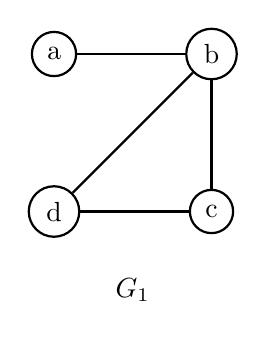
\begin{tikzpicture}
  \begin{scope}[every node/.style={circle,thick,draw}]
  \node (a) at (0,2) {a};
  \node (b) at (2,2) {b};
  \node (c) at (2,0) {c};
  \node (d) at (0,0) {d};
  \end{scope}
  \begin{scope}[every edge/.style={draw=black,thick}]
  \path (a) edge (b);
  \path (b) edge (c);
  \path (b) edge (d);
  \path (c) edge (d);
  \end{scope}
  \node () at (1,-1) {$G_1$};
  \end{tikzpicture}
  \hspace{1.5cm}
  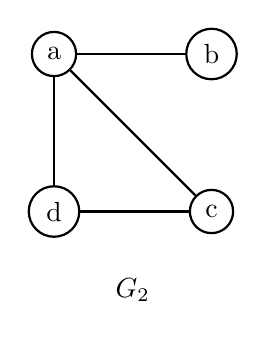
\begin{tikzpicture}
  \begin{scope}[every node/.style={circle,thick,draw}]
  \node (1) at (0,2) {a};
  \node (2) at (2,2) {b};
  \node (3) at (2,0) {c};
  \node (4) at (0,0) {d};
  \end{scope}
  \begin{scope}[every edge/.style={draw=black,thick}]
  \path (1) edge (2);
  \path (1) edge (3);
  \path (1) edge (4);
  \path (3) edge (4);
  \end{scope}
  \node () at (1,-1) {$G_2$};
  \end{tikzpicture}
  \caption{Nice pictures}
  \label{tikz:graphs}
\end{figure}


\begin{figure}
  \centering
  \begin{tikzpicture}[node distance=6cm]
  \node (a) [rect] {A Big Blue Block};
  \node (b) [oval, right of=a] {And His Oval Friend};
  \draw [line] (a) -- (b);
  \end{tikzpicture}
  \caption{Nice pictures}
  \label{tikz:graphs}
\end{figure}


\chapter{Technology Review}
About seven to ten pages.
\begin{itemize}

\section{J2EE}

\section{Heroku}

\section{MongoDB}

\section{SQL}

\section{Bootstrap}

\item Describe each of the technologies you used at a conceptual level. Standards, Database Model (e.g. MongoDB, CouchDB), XMl, WSDL, JSON, JAXP.
\item Use references (IEEE format, e.g. [1]), Books, Papers, URLs (timestamp) – sources should be authoritative. 
\end{itemize}

\section{XML}
Here's some nicely formatted XML:
\begin{minted}{xml}
<this>
  <looks lookswhat="good">
    Good
  </looks>
</this>
\end{minted}

\chapter{System Design}
As many pages as needed.
\begin{itemize}
\item Architecture, UML etc. An overview of the different components of the system. Diagrams etc… Screen shots etc.
\end{itemize}

\begin{table}[h]
  \centering
  \begin{tabular}{x{2cm}p{3cm}}
    \toprule \\
    Column 1 & Column 2 \\
    \midrule \\
    Rows 2.1 & Row 2.2 \\
    \bottomrule
  \end{tabular}
  \caption{A table.}
  \label{table:mytable}
\end{table}

\chapter{System Evaluation}
As many pages as needed.
\begin{itemize}
\item Prove that your software is robust. How? Testing etc. 
\item Use performance benchmarks (space and time) if algorithmic.
\item Measure the outcomes / outputs of your system / software against the objectives from the Introduction.
\item Highlight any limitations or opportuni-ties in your approach or technologies used.
\end{itemize}

\chapter{Conclusion}
About three pages.

\begin{itemize}
\item Briefly summarise your context and ob-jectives (a few lines).
\item Highlight your findings from the evalua-tion section / chapter and any opportuni-ties identified.
\end{itemize}

